\documentclass{article}
\usepackage{amsmath}
\usepackage{fancyhdr}
\usepackage{amssymb}
\usepackage{amsthm}
\usepackage{graphicx}
\usepackage{varioref}
\usepackage{verbatim} 
\usepackage{multicol}
\usepackage{enumerate}
\usepackage[normalem]{ulem}
%\usepackage[margin=1in]{geometry}
\usepackage{caption}
\usepackage{subcaption}
\usepackage[T1]{fontenc}
\usepackage[margin=1in]{geometry}
\usepackage{thm-restate}
\usepackage{enumitem}



\usepackage{mathrsfs}

\usepackage{url}\urlstyle{same}
\usepackage{xspace}
\usepackage{thm-restate}

% Nicer font
\usepackage{mathpazo}


% Microtype
\usepackage{microtype}

% TikZ
\usepackage{tikz}
\usetikzlibrary{calc}
\usetikzlibrary{decorations.pathmorphing}
\usetikzlibrary{decorations.markings}

% Support eps figures
\usepackage{epstopdf}

% Hypertext package
\usepackage[colorlinks = true]{hyperref}
% Title and authors
%\hypersetup{
%  pdftitle = {},
%  pdfauthor = {}
%}
% Color definitions
\usepackage{xcolor}
\definecolor{darkred}  {rgb}{0.5,0,0}
\definecolor{darkblue} {rgb}{0,0,0.5}
\definecolor{darkgreen}{rgb}{0,0.5,0}
% Color links
\hypersetup{
  urlcolor   = blue,         % color of external links
  linkcolor  = darkblue,     % color of internal links
  citecolor  = darkgreen,    % color of links to bibliography
  filecolor  = darkred       % color of file links
}

% Clever references
\usepackage{cleveref}%[nameinlink]
\crefname{lemma}{Lemma}{Lemmas}
\crefname{proposition}{Proposition}{Propositions}
\crefname{definition}{Definition}{Definitions}
\crefname{theorem}{Theorem}{Theorems}
\crefname{conjecture}{Conjecture}{Conjectures}
\crefname{corollary}{Corollary}{Corollaries}
\crefname{section}{Section}{Sections}
%\crefname{property}{Property}{Properties}
\crefname{appendix}{Appendix}{Appendices}
\crefname{figure}{Fig.}{Figs.}
\crefname{equation}{Eq.}{Eqs.}
\crefname{table}{Table}{Tables}
\crefname{claim}{Claim}{Claims}
%\crefname{item}{Property}{Properties}

%%%%%%%%%%%%%%%%%%%%%%%%%
%  N E W T H E O R E M  %
%%%%%%%%%%%%%%%%%%%%%%%%%

\newtheorem{theorem}{Theorem}
\newtheorem{lemma}[theorem]{Lemma}
\newtheorem{proposition}[theorem]{Proposition}
\newtheorem{definition}[theorem]{Definition}
\newtheorem{corollary}[theorem]{Corollary}
\newtheorem{conjecture}[theorem]{Conjecture}
\newtheorem{property}[theorem]{Property}
\newtheorem*{conjecture*}{Conjecture}
\newtheorem*{problem}{Problem}
\newtheorem{claim}[theorem]{Claim}
\theoremstyle{definition}
\newtheorem*{remark}{Remark}
\newtheorem*{example}{Example}

\DeclareMathOperator{\E}{\mathrm{E}}		     % expected value
\DeclareMathOperator{\p}{\mathrm{P}}		     % probability

\begin{document}


%+Title
\title{Applications of Graph Theory and Probability in the Board Game \it{Ticket to Ride}}

\author{R. Teal Witter \& Alex Lyford}

\date{\today}
%\date{\today}

\maketitle
%-Title

\section{Introduction}

\section{Background}
People have been playing mathematical games
since as early as 2000 B.C.
\cite{cornelius1986historical}.
From the beginning,
players have attempted to devise optimal
strategies, simulate future moves, or identify
flaws that can be exploited.
Mathematics can serve as a particularly powerful tool for
such analysis.
Abbott and Richey used Markov Chains
to find the long term 
distribution of turns players spend in different
properties in the board game
\textit{Monopoly} \cite{abbott1997take, magie1935}.
(They also found that the optimal strategy is to avoid making
moves altogether and instead maximize time spent in jail.)
Lyford et al. investigated the probability and expected value 
in the board game \textit{Camel Up}
\cite{bogen2014, lyford2019using}.
Witter and Lyford generated an optimal winning strategy for the 
board game \textit{Codenames} using matrix rotations
and a combinatorial argument \cite{chvatil2015}.
% TO DO: CITE CODENAMES PAPER IF ACCEPTED

Another example of a game with mathematical underpinnings is
the board game \textit{Ticket to Ride} \cite{moon2004ticket}. 
Players race to connect 
cities and build railroads on a map of the U.S.
Mathematically, the board
can be thought of as a graph where
cities represent vertices and the
routes between them represent edges.
The educational implications of \textit{Ticket to Ride}
have been extensively studied.
Lim applied the game to teach basic graph theory
\cite{lim2007taking}.
Chang et al. introduced Kruskal's, Prim's, and Dijkstra's
algorithms in the context of \textit{Ticket to Ride}
\cite{chang2008learning}.
Drake taught beginning programming skills by having
students implement a digital version of the game \cite{drake2011teaching}.
In addition, \textit{Ticket to Ride} has been studied in the context of
accessible game design and eye-tracking visualization
\cite{eriksson2005enhancing, newn2017evaluating}.

Previous work has also focused on improving player 
strategies in \textit{Ticket to Ride}.
Silva et al. used simulations to compare different
heuristic strategies (e.g. purchasing longest routes,
connecting all destination cards) \cite{de2017playtesting}.
In related papers, the same authors explore the 
game space to find trends in the way \textit{Ticket to Ride}
is played and experiment with new maps and decks 
\cite{de2017evaluator, de2018evolving}.

We extend the mathematical interpretations of
\textit{Ticket to Ride} to build on previous research
and devise better player strategies.
In particular, we apply expected value of collecting cards,
effective resistance, and betweenness centrality.

We rely on a well-known solution to the probability question:
"What is the expected number of cards until
we see three aces in a well-shuffled deck?"
We frame the problem of collecting the resources
to build a route in terms of the aces problem.
The solution gives us a proxy for the difficulty
of collecting routes.

In a graph, effective resistance corresponds
to the difficulty of an electrical current flowing
from one vertex to another.
We implement two existing algorithms to calculate
the effective resistances between cities
\cite{ellens2011effective, wu2004theory}.
By comparing the effective resistance to the reward
of collecting a pair of cities, we suggest an enhanced approach 
approach to picking destination cards.

Developed in 1977, betweenness centrality gives a measure
of the centrality of edges in a graph
\cite{freeman1977set}.
By calculating the edges with the highest betweenness centrality,
we enable players to pick the most central routes.
We compare the most theoretically central routes
to the ones owned by the winning player in Silva et al.'s
simulations \cite{de2017playtesting}.

The overarching question of this work is as follows:
What (if any) mathematical structure in \textit{Ticket to Ride}
can be exploited to optimize player strategies?
Our answer builds on existing results and
and our own novel applications of mathematical concepts to enhance
player strategies and propose a better scoring scheme.

\subsection{Ticket to Ride}
The goal is to collect as many points as possible before
any player uses all of their 45 trains and ends the game.
There are three ways players may earn points:
1) by building routes on the board
according to the number of trains in each route,
2) by building a path of routes
between two cities specified by a destination card in their possession,
3) by owning the longest continuous path of cities at the end of the game.

A player has three (mutually exclusive) options for what to do during
their turn:
1) draw train cards to build routes in later turns,
2) claim a particular route by returning the appropriate
number of trains of the specified color,
3) draw destination cards in order to earn points for connecting
distant cities.
\subsection{Strategy Assumptions}
We make several assumptions about how reasonable players
play \textit{Ticket to Ride}.
\section{Value of Routes}
\subsection{Current Route Value}
There are two factors that encourage players to buy longer routes:

- the reward per train is much higher for longer routes and

- only one route can be purchased per a turn so it is more efficient
to buy longer routes.

\begin{table}[h!]
\renewcommand{\arraystretch}{1.5}
\centering
\begin{tabular}{| c | c | c | c | c | c | c |}
\hline
 Route Length & 1 & 2 & 3 & 4 & 5 & 6\\
 \hline
 Points Scored & 1 & 2 & 4 & 7 & 10 & 15\\
 \hline
\end{tabular}
\caption{The current values of routes.}
\label{table:current_value}
\end{table}
From \cref{table:current_value} we see that 
the trains in the two shortest routes are each worth only one point
whereas the trains in the longest route are worth two and a half points.
The ostensible reason for the increasing value per train is that the
difficulty of collecting trains grows faster than the number of trains $k$.
The most intuitive way to quantify the difficulty of collecting $k$ trains
is the expected number of turns a player needs to collect them.
However, in \cref{sec:collecting_cards}, 
we show that the expected number of cards
until we get $k$ of a specific color is linear with $k$.

\subsection{Collecting Cards}\label{sec:collecting_cards}
Let $C$ be the set of all cards.
Our goal is to find the expected time until
we have collected $k$ of a specific
color of cards where $k$ is a fixed
integer between 1 and 6 inclusive.
Without loss of generality, say we are
looking for blue cards and
call $B$ the set of blue cards.
In order to find how long it takes to collect $k$ blue cards,
think of our well-shuffled deck as
blue cards separated by non-blue cards.
For example, we may have the ordering
\begin{align}
    xxxbxbxxxx...xxbxxx \nonumber
\end{align}
where $x \in C \setminus B$ and $b \in B$.

Now let $T$ be the number of cards until
the $k^{th}$ blue card is drawn.
Our strategy is to write $T$ in terms of $k$
and indicator random variables.
Let $I_x$ be the indicator that takes value 1
if non-blue card $x$ appears before the $k^{th}$ blue card
and 0 otherwise.
Then
\begin{align}
    T = k + \sum_{x \in C \setminus B} I_x. \nonumber
\end{align}

We are interested in the average number of draws
until we see $k$ blue cards
so we take the expected value of $T$
(distributing expectation over addition),
\begin{align} \label{eq:expected_card}
    \E[T] = \E[k] + (|C \setminus B|) \E[I_x].
\end{align}
We know that $k$ is fixed so its expected value is simply $k$.
Then the only unknown is $\E[I_x]$.

To find $\E[I_x]$ think of the deck as 13 sequences 
of non-blue cards where adjacent sequences are
separated by a single blue card.
(It is possible for a sequence to be of length zero provided
two blue cards are adjacent to each other.)
Since we assume the deck is well-shuffled, the non-blue cards
are uniformly distributed across each sequence;
it is as likely for card $x$ to be in any one sequence
as any other.

Now think of whether a card appears before the $k^{th}$ blue
in terms of which sequence it lives in.
Card $x$ appears before the first blue if and only if it is 
in the first sequence.
The probability $x$ is in the first sequence is $1/13$
so $x$ appears before the first blue with $1/13$ probability.
(Recall that $x$ is uniformly distributed across all
13 sequences.)
Similarly, card $x$ appears before the $k^{th}$ blue if and only if
it is in one of the first $k$ sequences.
The probability $x$ is in the first $k$ sequences is $k/13$
so $x$ appears before the $k^{th}$ blue with $k/13$ probability.
By conditioning on whether $x$ appears before the $k^{th}$ blue,
we may write
\begin{align} \label{eq:expected_indicator}
    \E[I_x] &= 1 \times 
    \p(\textrm{$x$ appears before the $k^{th}$ blue}) +
    0 \times \p(\textrm{$x$ appears after the $k^{th}$ blue})
    \nonumber \\
    &= \p(\textrm{$x$ appears before the $k^{th}$ blue})
    = k/13.
\end{align}

With \cref{eq:expected_card} and \cref{eq:expected_indicator},
\begin{align}
    \E[T] &= k + (|C \setminus B|) k/13 \nonumber \\
    &= k \left(1 + \frac{|C| - |B|}{13}\right). \nonumber
\end{align}

\subsection{Converting Cards to Turns}\label{sec:converting}
\section{Effective Resistance \& Destination Tickets}

\begin{figure*}[!ht]
\centering
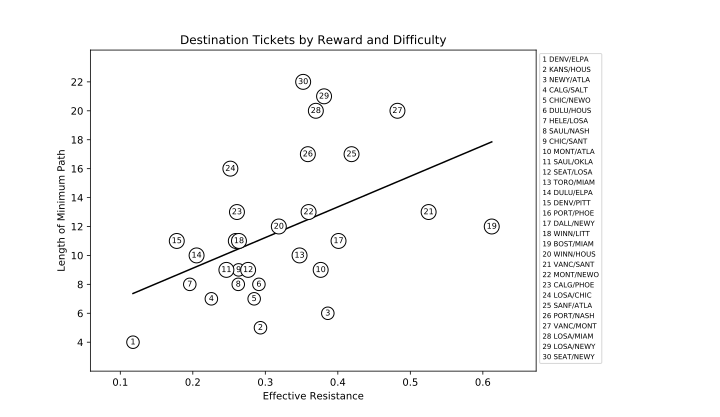
\includegraphics[scale=.8]{figures/resistance}
\caption{Destination Tickets by their effective
resistance and minimum path length.
The line of best fit gives an approximation of the
Destination Tickets that are better than average (above the line)
and worse than average (below the line) in terms
of the point value per difficulty.
Note: the $16^{th}$ Destination Ticket Portland/Phoenix is obscured
by the $18^{th}$.}
\label{fig:resistance}
\end{figure*}

\subsection{Simulations}

\begin{figure*}[!ht]
\centering
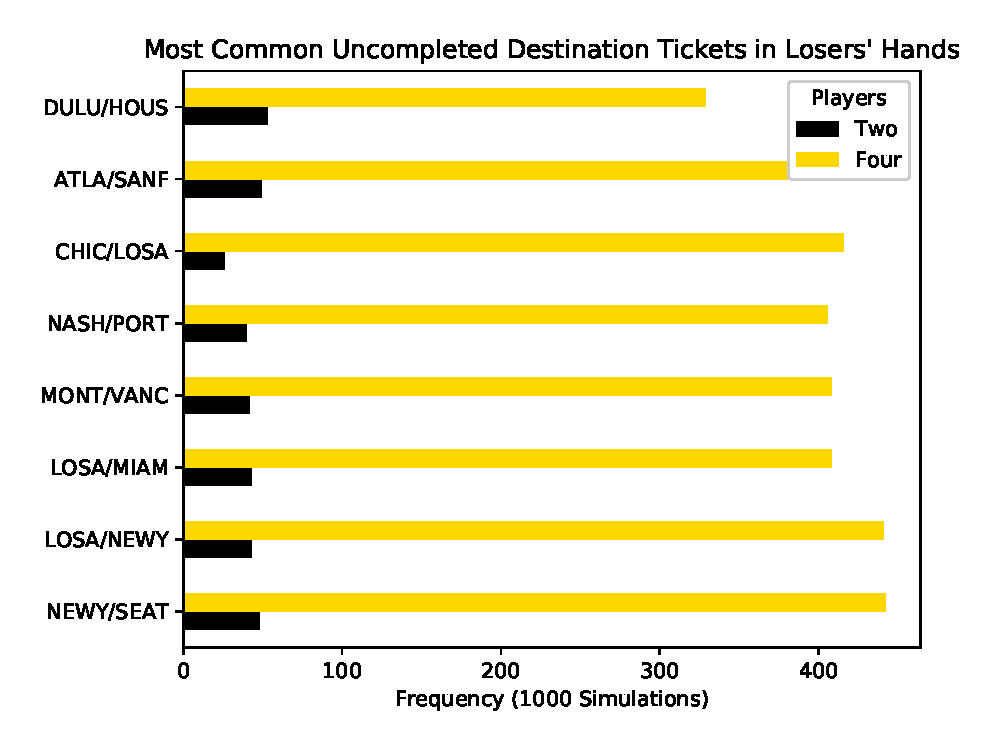
\includegraphics[scale=.8]{figures/uncompleted}
\caption{The most common uncompleted
Destination Tickets in the losers'
hands at the end of 1000 simulated games.
The disparity between two and four player
games originates from the different number
of losers: most of the time there are three 
losers in the four person game whereas there is 
always only one loser in the two person game.
(Games were simulated using
Silva et al.'s code.)}
\label{fig:uncompleted}
\end{figure*}

\begin{figure*}[!ht]
\centering
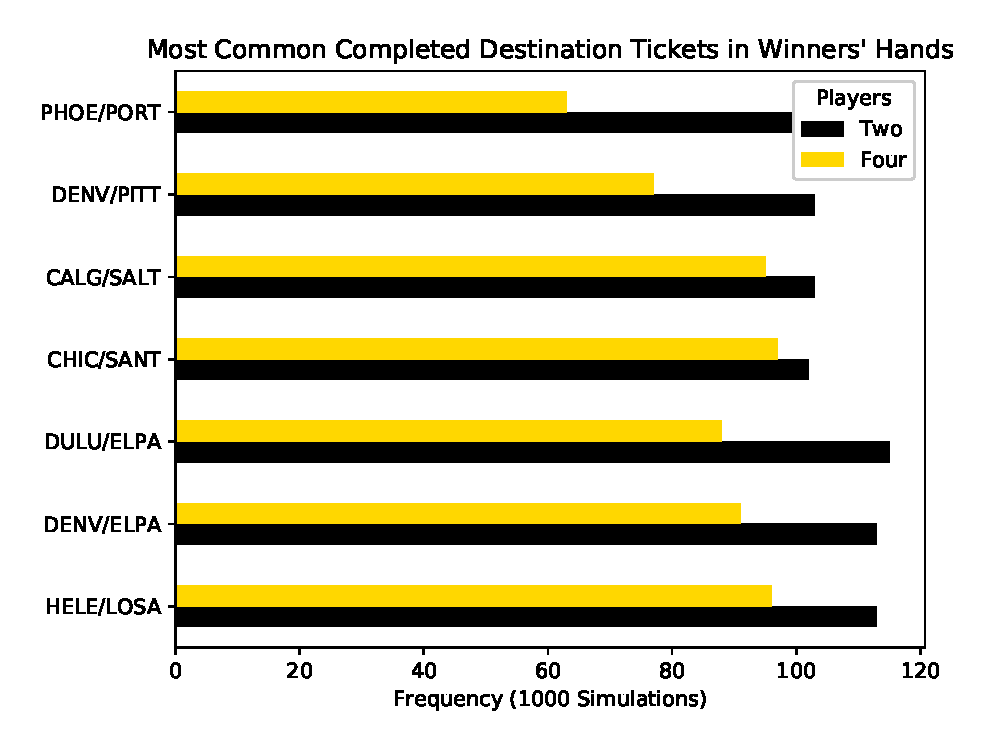
\includegraphics[scale=.8]{figures/completed}
\caption{The most common completed
Destination Tickets in the winners'
hands at the end of 1000 simulated games.
(Games were simulated using Silva et al.'s code.)}
\label{fig:completed}
\end{figure*}
\section{Betweenness Centrality}

\subsection{Simulations}

\begin{figure*}[!ht]
\centering
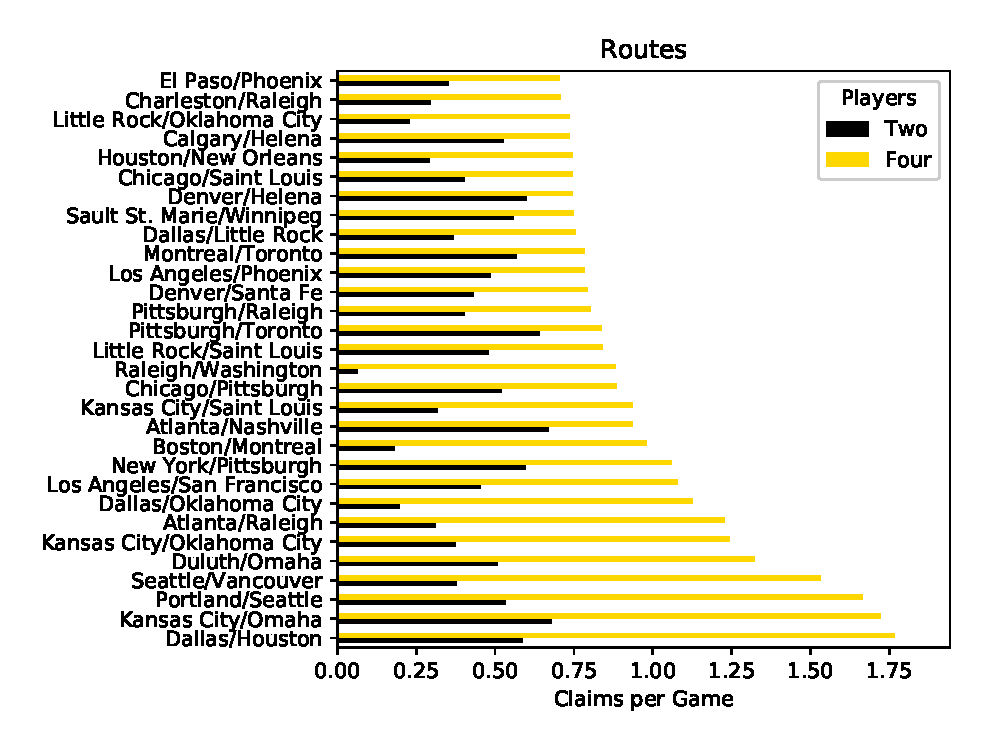
\includegraphics[scale=.8]{figures/routes}
\caption{The most common routes in the winning
player's hand at the end of
1000 simulated games.
(Games were simulated using Silva et al.'s code.)}
\label{fig:routes}
\end{figure*}

\bibliographystyle{abbrv}
\bibliography{main}

\end{document}
